\documentclass[12pt,a4paper]{article}
\usepackage{graphicx}
\usepackage[catalan]{babel}
\usepackage[utf8]{inputenc}
\usepackage[T1]{fontenc}
\usepackage{times}
\usepackage{amsmath}
\usepackage{listings}
\usepackage{amssymb}
%\usepackage{geometry}
\usepackage{url}
\newcounter{exercises}
\setcounter{exercises}{0}
\newtheorem{exer}[exercises]{Pregunta}
\newtheorem{exers}{Exer}
\usepackage{color}


%\geometry{a4paper,tmargin=25mm,bmargin=25mm,lmargin=25mm,rmargin=25mm}

%\pagestyle{empty}

\begin{document}

\section*{Xarxes d’Ordinadors i Internet \\ Curs 2023-2024}
\section*{Pràctica 1: \textit{Simulacions de Xarxa: Protocols de capa física i d'enllaç de dades.}}

\vspace*{0.5cm}
\section{Introducció}


\subsection*{Protocols de xarxa}
L'existència de xarxes de computadors és possible gràcies a la combinació de diversos protocols de comunicació, aquests protocols estableixen un conjunt de conceptes comuns que permeten l'intercanvi de dades entre tota mena de dispositius de xarxa. Aquests protocols s'organitzen en capes i s'agrupen en forma de pila. Les dues classificacions més utilitzades són el model OSI (Open Systems Interconnection) \cite{osi} i el model estàndard que s'utilitza a Internet, la pila de protocols TCP/IP \cite{internet}.

\begin{figure}[!ht]
  \begin{center}
    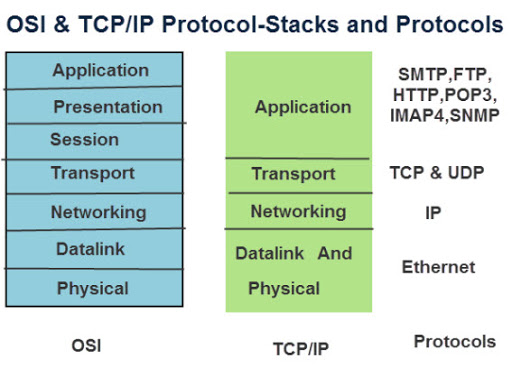
\includegraphics[width=0.7\textwidth]{protocol-stack}
    \caption{Comparativa de les piles - ISO i TCP/IP}
    \label{osi-stack}
  \end{center}
\end{figure}

Les capes inferiors gestionen conceptes del medi físic (freqüències d'ona, modulació, etc.), a mesura que anem pujant de capa els protocols defineixen conceptes més abstractes, com poden ser el format o l'ordre dels missatges. Finalment el nivell més alt (capa d'aplicació) serà en el que se situarien les aplicacions de software que utilitzem comunament (navegadors, client de correu, etc.). Aquest model aporta gran flexibilitat, ja que permet la comunicació de dispositius sempre que comparteixin el mateix protocol a la capa superior, independentment de la tecnologia utilitzada a les capes inferiors.

En aquesta pràctica ens centrarem en les capes físiques i d'enllaç de dades, estudiarem diversos escenaris de xarxa amb dispositius i medis variats, i analitzarem el comportament dels protocols que s'utilitzen en cada cas. Per fer aquesta pràctica utilitzarem dos tipus d'eines, un simulador de xarxa i un analitzador de tràfic

\subsection*{Simuladors de Xarxa}
% TO DO Millorar
Els simuladors de xarxes són programes que modelen el comportament de les xarxes, ja sigui a través de models matemàtics o a través de l'observació directa del tràfic o de les traces generades. Els simuladors permeten predir el funcionament d'una xarxa en funció d'una sèrie d'atributs de l'entorn que es poden modificar. A nivell d'administració de xarxes, l'ús de simuladors és molt útil per estudiar els efectes de les futures ampliacions o modificacions que pugui patir una xarxa.

% En l'àmbit acadèmic, els simuladors també són molt utilitzats per a mesurar i predir el rendiment de nous protocols, sistemes o topologies i comparar-los amb d'altres existents sense necessitat d'implementar físicament tots els canvis. D'aquesta forma, s'aconsegueix un gran estalvi en temps i diners.


%%%%%%%%%%%%%%%%%%%%%
% OPNET
%%%%%%%%%%%%%%%%%%%%%

En aquesta pràctica utilitzarem Network Simulator 3 (NS-3) \cite{ns3}. Aquest és un simulador de xarxa per a entorns Linux que ofereix una API amb la qual es poden crear scripts de simulació en llenguatge C++ o Python. El simulador s'executa com aplicació de consola, però en cas de desitjar-ho tenim la possibilitat de visualitzar els resultats mitjançant una GUI. NS-3 suporta totes les tecnologies de xarxa més habituals (Ethernet, LTE, WiFI, etc\dots) i disposa de models per cada tecnologia. A l'hora de configurar-lo, tots els elements es basen en una llista d'atributs sobre la qual tenim un gran control.

% Riverbed Modeler recull qualsevol tipus d'informació (és molt configurable) sobre les simulacions que executem, a més, realitza gràfics i estadístiques sobre aquesta informació i permet fer comparacions molt fàcilment. Com que utilitzarem una llicència acadèmica, la quantitat de tràfic que podem simular és limitada (no més d'una hora de funcionament).

\subsection*{Analitzadors de paquets}
Un analitzador de paquets és un programa informàtic que captura les trames generades en una xarxa d'ordinadors. A més fa una conversió del tràfic de xarxa en un format entenedor pels humans i mitjançant la seva interficie gràfica  ens permet visualitzar aquesta informació de forma simple.

En aquesta pràctica utilitzarem Wireshark \cite{wireshark}. Wireshark és un programari lliure i de codi obert programat en C++ que inclou les funcionalitats de captura i visualització de paquets. El farem servir principalment per visualitzar el tràfic de xarxa generat a les simulacions de NS-3.

\subsection*{Encapsulat de dades}

Tota informació transmesa a través de xarxa fent servir els protocols de la pila TCP/IP segueix un procés d'encapsulació. El protocol que es faci servir a cada capa defineix una estructura de dades que serà la unitat bàsica de transferència d'informació per aquella capa. Aquesta unitat bàsica sempre inclourà les dades que es volen transferir per la capa superior, més un conjunt de meta-dades que són necessaris pel correcte funcionament d'aquesta capa. Aquestes meta-dades poden incloure conceptes com: informació d'adreçament (per saber destinació i origen), números de seqüència (per poder establir l'ordre en què arriben les dades), codis de detecció d'errors, etc. Aquestes meta-dades sempre s'annexen per davant (header) o per darrere (trailer). Per entendre com funciona l'encapsulació observeu la \textbf{Figura \ref{encapsulation}}, es mostra una aplicació que vol transmetre dades mitjançant TCP/IP:

\begin{enumerate}
 \item Les dades de l'aplicació es passaran a la capa de transport (4), per garantir fiabilitat de transmissió es farà servir el protocol TCP, que encapsularà les dades afegint les seves capçaleres, això formarà l'estructura bàsica de dades de capa 4, anomenada \textbf{Segment}. 
 \item El segment es passarà a la capa inferior (3). En aquest cas el protocol d'aquesta capa (IP) afegirà les seves capçaleres al segment i formarà la unitat bàsica de capa 3, anomenat \textbf{Datagrama}.
 \item El datagrama es passarà a la capa inferior (2), el protocol encarregat d'aquesta capa (Ethernet) afegirà les seves dades i formarà la unitat bàsica de capa 2, el frame \textbf{Frame}.  Són aquests Frames (amb les meta-dades afegides per les capes superiors) els que s'envien a través del medi de transmissió. 
  
\end{enumerate}
%Aquest proces es troba representat a la \textbf{Figura \ref{encapsulation}}.

\begin{figure}[!ht]
  \begin{center}
    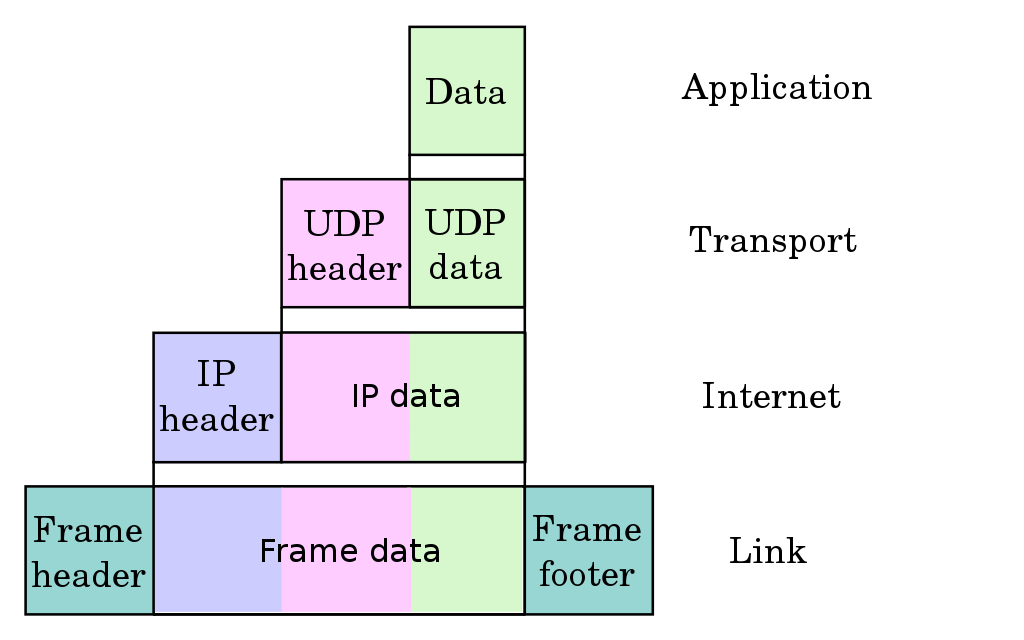
\includegraphics[width=0.615\textwidth]{encapsulation}
     \caption{Encapsulat de dades d'aplicació descendent a través de les capes.}
    \label{encapsulation}
  \end{center}
\end{figure}

\newpage
\begin{figure}[!ht]
Entre les diferents funcionalitats disponibles a \textbf{Wireshark} disposem d'un visualitzador de contingut de trames (vegeu Figura \ref{wireshark-frame}). Això ens permet veure un desglossat dels diferents camps que composen un Frame capturat, incloent-hi les capçaleres afegides per cadascun dels protocols de les capes superiors.
  \begin{center}
    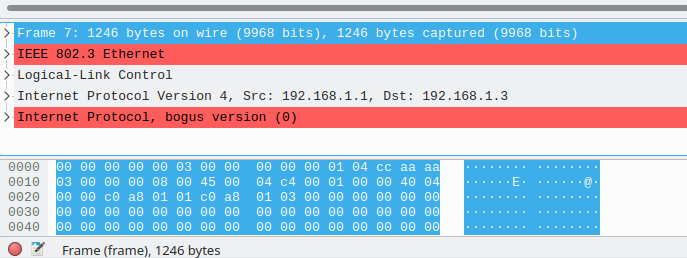
\includegraphics[width=1\textwidth]{wireshark-frame}
    \caption{Wireshark: visualització de contingut de trames.}
    \label{wireshark-frame}
  \end{center}
\end{figure}



\section*{Observacions}

%  \begin{tabular}{||p{12cm}||}
%  \hline\hline
 \begin{itemize}
 \item Aquesta pràctica es divideix en dues parts: una part teòrica, que es realitza com a treball previ en forma de qüestionari, i una part experimental a dur a terme durant les sessions de laboratori.
 \item La part experimental es desenvolupa en grups de 2 durant un total de 3 sessions, seguint un guió que inclou diversos experiments que \textbf {s'han de completar durant la mateixa sessió.} Posteriorment, amb els resultats obtinguts, es respondran quatre preguntes, les quals caldrà \textbf{lliurar a través del campus virtual el mateix dia de la pràctica}.
\item La part experimental inclou elements que es generen aleatòriament i són únics per a cada grup, fent que la resposta correcta variï en cada cas. A cada lliurament a través del campus virtual, se us demanarà proporcionar el vostre identificador per detectar la permutació que correspongui a les vostres preguntes. En cas de detectar més d'un lliurament amb el mateix identificador, es considerarà plagiat i \textbf{tots els grups implicats suspenderan les pràctiques automàticament}.
\item L'última sessió experimental de pràctiques es realitzarà individualment amb el propòsit de verificar que tots els membres del grup han assolit els coneixements esperats. Aquesta sessió constarà de 3 preguntes, de les quals s'hauran d'encertar com a mínim 2 per aprovar la pràctica.
\item Cada sessió de pràctiques comptabilitza a la nota final. Les absències s'hauran de recuperar assistint a un altre grup de pràctiques, o bé assumir la pèrdua de puntuació que correspongui a aquella sessió.
 \item Aquesta pràctica es realitza dins de la màquina virtual \textbf{Xarxes}, la qual trobareu a l'escriptori dels ordinadors del laboratori. Podeu iniciar sessió amb les següents credencials:
\newline \texttt{usuari:} \textbf{alumne}
\newline \texttt{password:} \textbf{alumne}
\item Per aquesta pràctica, necessitareu fer servir la consola de sistema. Podeu accedir-hi fent clic a \textbf{Home} $\rightarrow$ \textbf{Terminal Emulator} o bé fent clic dret a l'escriptori i seleccionant \textbf{Open Terminal Here} al menú contextual.

\item Per aquesta pràctica, es recomana situar el vostre terminal al directori: \newline \textbf{/home/alumne/practiques/practica1/} (feu servir la comanda \textbf{cd}). A dins, trobareu la següent estructura de directoris:
\begin{itemize}
\item\textbf{simulation-scripts}: Aquí trobareu els scripts de simulació a utilitzar durant la pràctica.
\item\textbf{exam}: Inclou un enunciat personalitzat que cada membre del grup haurà de respondre de forma individual (apareixerà únicament el dia de la prova de validació).
%\item\textbf{informe}: Carpeta on heu de desar els arxius abans de generar el zip del lliurament.
\end{itemize}

\item El contingut de la carpeta \textbf{simulation-scripts} es restaura cada cop que tanqueu sessió. Qualsevol modificació als scripts originals es perdrà. Això només s'aplica als arxius originals. Per tant, si necessiteu realitzar algun canvi de forma persistent, haureu de desar-ho com un nou arxiu amb un nom diferent.

\item Cada execució del simulador generarà diversos fitxers amb extensió \textbf{pcap}. Podeu visualitzar-los amb \textbf{Wireshark}, simplement fent doble clic a l'arxiu dins de l'explorador de directoris.

\item El format de les pràctiques consisteix en realitzar els experiments descrits al guió de pràctiques.
\end{itemize}
%  \\\hline\hline
%  \end{tabular}
%  \medskip

 \newpage
\section {Qüestionari previ}

Busqueu informació i responeu breument a les següents preguntes:
\begin{itemize}
\item \begin{exer}Que és un medi de transmissió? Enumera els 2 tipus de medi més comuns.\end{exer}
\item  \begin{exer} Quin és el proposit del component hardware anomenat NIC?\end{exer}
% \item \begin{exer}Que és un cable CAT6? De forma comú amb quin protocol de Capa 2 es fa servir aquest cable?
% Llista 2 tipus de cable d'aquesta mateixa classificació i comenta les diferencies.\end{exer}
% \item Que és un cable creuat? Quina utilitat tenia aquesta tipus de cable?
\item \begin{exer}Que és un Hub?, i un Switch? A quina capa del model de xarxa treballa cadascun d'aquests dispositius? Llisteu les principals diferències.\end{exer}
\item \begin{exer}Que és un domini de col·lisió ? Quants dominis de col·lisió té una xarxa amb un Hub?, i una amb un Switch?\end{exer}
\item \begin{exer} Quin és el propòsit del protocol CSMA? Perquè creieu que és especialment important en una xarxa amb un Hub?\end{exer}
\item \begin{exer} Com es diu la variant de CSMA que es fa servir en xarxes Ethernet?, i la que es fa servir en xarxes WiFi? En què es diferencien? \end{exer}
\item \begin{exer} Tenint en compte el funcionament de CSMA: en cas que un node afegeixi dades a la seva cua de transmissió abans que un altre, transmetrà \textbf{sempre} les seves dades abans que aquest altre? \end{exer}
\item \begin{exer} Que és un Acces Point (AP)?\end{exer}
\item \begin{exer} Que és un SSID? \end{exer}
\item \begin{exer} Que és el protocol WiFi? A quina capa de la pila de protocols se situa? En un context de xarxa amb cables, quin seria el protocol més similar?\end{exer}
\item \begin{exer} Que és un Management Frame, llisteu els tipus de management frame i expliqueu quin propòsit té cadascun d'ells. \end{exer}
\item \begin{exer} Que és una adreça MAC? i una adreça IP? A quina capa de protocol s'utilitzen aquest tipus d'adreces? \end{exer}
\item \begin{exer} Que és una adreça de broadcast, quina és l'adreça MAC de broadcast? \end{exer}
\item \begin{exer} Que és el protocol ARP? A quin nivell de capa correspon? Per a què s'utilitza? Per quin motiu es fa servir l'adreça MAC de broadcast a dins del protocol ARP?  \end{exer}
\item \begin{exer} Busqueu informació sobre l'aplicació de linía de comandes \textbf{ping}, quin tipus de protocol de xarxa fa servir aquesta aplicació? \end{exer}
\item \begin{exer} Que és un router? A quina capa actua un router? \end{exer}
\item \begin{exer} Que és la MTU d'una xarxa? Quin procés es du a terme quan es vol transmetre un paquet
que excedeix la MTU?\end{exer}
\end{itemize}

El lliurament d'aquestes preguntes s'ha de fer a través del qüestionari moodle: \textbf{Qüestionari previ pràctica 1} que trobareu al campus virtual. La data límit de lliurament és la segona setmana de pràctiques \textbf{(Dijous 29/03/24)}, però és \textbf{molt recomanable} haver finalitzat fins a la \textbf{pregunta 7} abans de la primera sessió de laboratori.

\section{Guió de la pràctica}

\subsection{Configuració inicial}
La primera vegada que utilitzeu l'entorn de pràctiques, serà necessari especificar la informació del vostre grup. \textbf{Aquest pas s'ha de realitzar a l'inici de cadascuna de les sessions de pràctiques}:
\begin{itemize}
 \item Obriu un terminal, proporcioneu la informació que us demani el sistema (això només es demanarà la primera vegada que es fa servir aquest entorn, si no us surt això, haureu de restaurar l'entorn, s'explica una mica més endavant).
     \newline 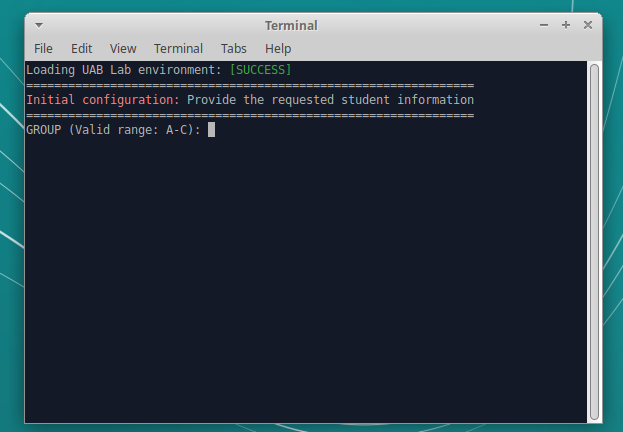
\includegraphics[width=0.85\textwidth]{ubuntu5}
 \item Un cop introduides les vostres dades l'entorn quedarà configurat, a partir d'aquest moment els resultats experimentals que obtingueu seran exclusius pel vostre grup.
 \item Ara es necessari que executeu la següent comanda per obtenir el vostre identificador de grup:
 \begin{lstlisting}[language=bash,basicstyle=\footnotesize]
   echo $USR_REF
\end{lstlisting}
 \item En pantalla apareixerà un identificador de 15 caràcters que permet identificar les combinacions de preguntes assignades al vostre grup. \textbf{És crucial que prengueu nota d'aquest valor, ja que haureu de proporcionar-lo en cada lliurament a través del campus virtual.}

 \item Com que els ordinadors són compartits, és possible que algun grup hagi realitzat la configuració de l'entorn prèviament. Podeu verificar si l'entorn està configurat amb la informació d'un altre grup amb la comanda següent:
  \begin{lstlisting}[language=bash,basicstyle=\footnotesize]
   echo $GRUP$SUBGRUP
\end{lstlisting}
 \item Si les dades no coincideixen amb les vostres, haureu d'executar:
   \begin{lstlisting}[language=bash,basicstyle=\footnotesize]
   get-student-info.sh -p
\end{lstlisting}
\item Tanqueu el terminal i torneu-lo a obrir. Ara hauria de sortir el menú de configuració d'entorn inicial.
\end{itemize}


\subsection{Xarxes locals cablejades}

El Hub i el Switch són els dispositius que es fan servir per crear xarxes locals cablejades. A continuació analitzarem de forma pràctica com es diferencien.
\begin{enumerate}
\item Obriu la carpeta \textbf{simulation-scripts} i localitzeu els arxius: \textbf{hub-scenario.cc} i \textbf{switch-scenario.cc}. Obriu-los amb un editor de text per visualitzar el contingut.

Aquests scripts descriuen una xarxa d'ordinadors fent servir programació orientada a objectes mitjançant l'API que proporciona el simulador ns-3. No és necessari que entengueu tot el que es fa a l'script, però sí que tingueu una idea general.
%, a l'annex \ref{} es desglossa en detall la funcionalitat de cada objecte. 

Aquests scripts defineixen una xarxa local Ethernet amb diversos ordinadors (numerats incrementalment començant per 1, on \textbf{n1} seria el \textbf{Node 1}, etc.) connectats per cables. En una de les xarxes, s'utilitza un  \textbf{hub} com a dispositiu central, mentre que en l'altra es fa servir un  \textbf{switch}. A tots els nodes de les dues xarxes se'ls instala un stack de protocols TCP/IP. A més, hi ha dues parelles de nodes que intercanviaran tràfic de forma intermitent mitjançant una aplicació \textbf{OnOff}. Finalment, es defineix que la simulació té una durada de 6 segons.
\item Obriu una consola i executeu la següent comanda:
%\begin{minted}{bash}
\begin{lstlisting}[language=bash,basicstyle=\footnotesize]
ns3-run-wparams "externals/hub-scenario" --vis --equalize
\end{lstlisting}
%\end{minted}

\begin{figure}[!ht]

  \begin{center}
  \label{simulator}
    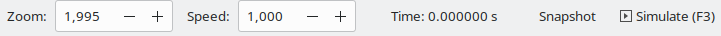
\includegraphics[width=1\textwidth]{simulator}
    \caption{Controls del visualitzador de simulació}
  \end{center}
\end{figure}
Això us obrirà una finestra de visualització on podreu observar la xarxa gràficament. A la part inferior de la finestra podreu veure el panell de control (Figura 4).

\begin{itemize}
 \item Feu clic al botó \textbf{Simulate}.
 \item Executeu la simulació fins a que el comptador \textbf{Time} arribi a 6.0 s
\end{itemize}

Això us permetrà observar la comunicació entre les parelles de nodes.

\item A continuació repetiu la mateixa prova amb l'scenari switch:
%\begin{minted}{bash}
\begin{lstlisting}[language=bash,basicstyle=\footnotesize]
ns3-run-wparams "externals/switch-scenario" --vis --equalize
\end{lstlisting}

\item Fixeu-vos en les diferències visuals entre els dos escenaris. Podem apreciar que en l'escenari hub, el node central no queda representat a la simulació. Això es deu al fet que es tracta d'un dispositiu de capa física que no interpreta trames de dades, i per tant, es representa simplement com un mitjà de transmissió.
\begin{figure}[!ht]
  \begin{center}
    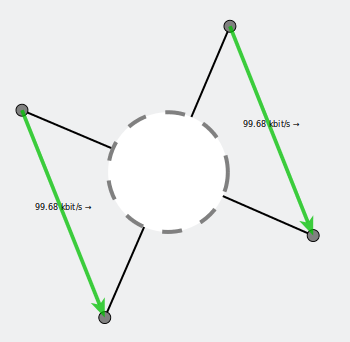
\includegraphics[width=0.4\textwidth]{hub-coms}
    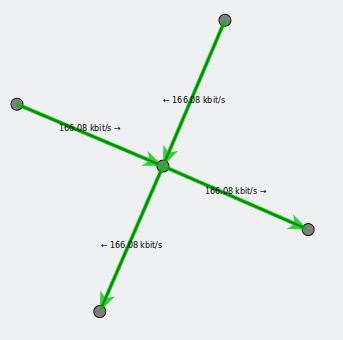
\includegraphics[width=0.4\textwidth]{switch-coms}    
    \label{ns3}
  \end{center}
  \begin{center}
   Nota: El nombre de nodes de la figura i el que observeu vosaltres pot variar.
  \end{center}

\end{figure}
% \begin{exer} Perquè creieu que els nodes de l'escenari Hub es comuniquen sense que aquest dispositiu aparegui a la simulació? Amb quin dels trets diferenciadors esmentats a la Pregunta 4 associaríeu aquest fet? \end{exer}
\item Identifiqueu els dos nodes que actuen com a origen de dades observant quin dels nodes mostra una fletxa sortint. Passeu el cursor del ratolí sobre ells per visualitzar la seva informació i preneu nota dels seus números, ja que els necessitareu més endavant.
\newline \begin{center} 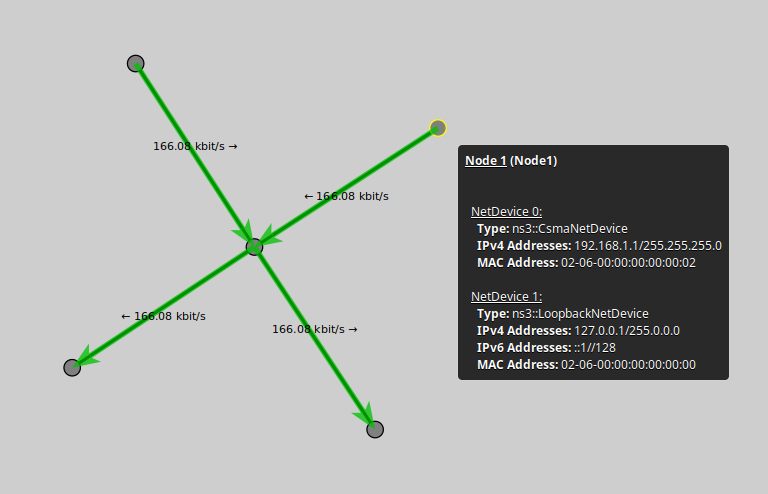
\includegraphics[width=0.6\textwidth]{hub-select} \end{center}
\item Un cop tancada la simulació, si observeu el directori on heu executat les simulacions, veureu que s'han generat múltiples fitxers \textbf{.pcap}. Aquests fitxers segueixen la sintaxi \textbf{<nom-scenari>-<NodeN>-0.pcap}. Cada arxiu conté el tràfic rebut per la NIC del node especificat. Per analitzar el contingut dels arxius podeu fer servir \textbf{Wireshark}.

Als arxius de traces apareixerà el tràfic generat per tots els protocols de l'stack TCP/IP, per aquest experiment ens interessa veure exclusivament els paquets generats per les aplicacions \textbf{OnOff}. Feu servir la barra de filtre de \textbf{Wireshark} per excloure els continguts no desitjats (Figura 5):

\begin{figure}[!ht]
  \begin{center}
    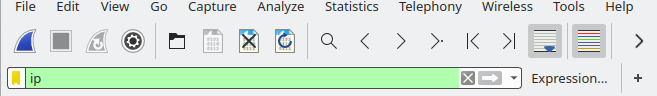
\includegraphics[width=1\textwidth]{wireshark-filter}    
    \label{wireshark-filter}
    \caption{Barra del filtre de Wireshark}
  \end{center}
\end{figure}

En ambdós escenaris tenim la mateixa situació: dues parelles de nodes que intercanvien dades. Tot i això, si observem el tràfic de cada node, apreciarem diferències. Compareu els arxius de tràfic de cada node de l'escenari Hub amb el seu homònim de l'escenari Switch.

\begin{exer} Quins són els nodes emissors de l'escenari Switch? Quin tràfic podem observar als nodes de l'escenari Hub però no als del Switch? Amb quin dels trets diferenciadors entre un hub i un switch associaríeu aquest fet? \end{exer}

Obriu novament al codi font dels scripts de simulació: \textbf{hub-scenario.cc} i \textbf{switch-scenario.cc}. Podreu apreciar que l'escenari Hub fa servir un canal CSMA compartit entre els 4 nodes. Per altra banda l'escenari Switch fa servir un canal diferent per cada Node connectat al switch.

\begin{exer} A partir d'aquesta observació, amb quina característica dels hubs/switches podríem associar el CSMA-channel? \end{exer}

A continuació observarem el funcionament del protocol CSMA, executeu la següent comanda:

\begin{lstlisting}[language=bash,basicstyle=\footnotesize]
   ns3-run-wparams "externals/hub-scenario" -printChannelState
\end{lstlisting}
Això habilita les traces de log associades al medi físic i al protocol CSMA. Observeu els missatges que han aparegut per consola, les traces segueixen el següent format:
$$
a. Objecte  - b. Esdeveniment - c. Parametres - d. Temps $$

\begin{enumerate}
\item Objecte: Indica quin és l'objecte al qual correspon aquest Esdeveniment, podrà ser un Node concret o bé el canal de comunicació (cable).
\item Esdeveniment: Indica quin tipus d'esdeveniment ha ocorregut. Els esdeveniments portaran el sufix \textbf{Phy} si es corresponen a un esdeveniment de capa física o \textbf{Mac} per capa d'enllaç. Tingueu en compte també les següents abreviatures: Tx = Transmit i Rx = Receive.
\item Paràmetres: Informació addicional que pugui ser rellevant per aquest esdeveniment concret.
\item Temps: instant de simulació en el que ha ocorregut aquest esdeveniment.
\end{enumerate}

Tenint en compte que \textbf{MacTx} és l'esdeveniment en el qual un frame s'afegeix a la cua de transmissió de la NIC i \textbf{PhyTx} és el moment en què la NIC transmet els senyals elèctrics a través del cable de xarxa, Responeu:
\begin{exer} Doneu la llista ordenada de nodes que han enviat informació durant la simulació (si envien informació diversos cops llisteu-los múltiples vegades). \end{exer}
\begin{exer} Heu detectat algun cas en què la transmissió de dades no s'hagi produït immediatament? En cas afirmatiu, llisteu la primera ocurrencia.
Heu detectat algun cas en què a un node que es troba en espera se li hagi colat un altre al davant? En cas afirmatiu, llisteu la primera ocurrencia.\end{exer}
% \begin{exer} Quin és el propòsit de l'exponential backoff? Quin impacte creieu que té en l'ordre en què transmeten els nodes? \end{exer}
% \item Podriem crear una xarxa sense fer servir un d'aquest dispositius? En cas afirmatiu, dona 2 exemples de com ho podriem fer (pista: no totes les xarxes fan servir cables).
\end{enumerate}


\subsection{Xarxes locals sense fils}
A continuació donarem un cop d'ull a les característiques i protocols d'una xarxa sense fils, concretament un escenari WiFi.
\begin{enumerate}

\item Obriu la carpeta \textbf{simulation-scripts} i localitzeu l'arxiu: \textbf{wifi-scenario.cc}. Obriu-lo amb un editor de text per visualitzar el contingut.

En aquests scripts es defineix una xarxa local WiFi amb múltiples ordinadors (numerats incrementalment començant per 1). S'utilitza un \textbf{Acces Point (AP)} com a dispositiu central. A tots els nodes se'ls instala un stack de protocols TCP/IP. Addicionalment, a dos dels nodes se'ls instala una aplicació que genera tràfic de xarxa de forma intermitent (\textbf{OnOff}). Finalment, es defineix que la simulació té una durada de 6 segons.

Com podeu observar l'escenari té una configuració equivalent a la que fèiem servir als escenaris de xarxa cablejada.

Executeu la següent comanda i deixeu córrer la simulació fins al final:
\begin{lstlisting}[language=bash,basicstyle=\footnotesize]
ns3-run-wparams "externals/wifi-scenario" --vis
\end{lstlisting}

% \item \begin{exer} El fet de no estar lligats amb un cable confereix als nodes una propietat que abans no tenien, podríeu dir quina és?
%(Pista: És un tret visualment observable i no té un caire tècnic). \end{exer}

\item Si observeu el directori on heu executat la simulació veureu que s'ha generat el fitxer. \textbf{wifi-scenario-AccesPoint-0.pcap}, com a punt
central de la xarxa en aquest fitxer trobarem tot el tràfic generat pels nodes wireless. Obriu-lo amb wireshark i apliqueu el següent filtre:

$$ wlan.fc.type == 0 $$ 
Això us mostrarà un tipus de tràfic exclusiu de les xarxes wifi que es diuen \textbf{Management Frames}.

\item Mireu amb detall el contingut de la columna \textbf{Info} per identificar el tipus de management frame que correson a cada paquet.

\begin{exer} Quin és el rol que desenvolupa el node que envia Management Frames de tipus \textbf{Beacon}? Indiqueu la seva adreça MAC.\end{exer}

\begin{exer} Indiqueu l'adreça MAC del primer node que s'ha afegit a la xarxa Wifi (Pista: Raoneu quins tipus de management frame són necessaris per registrar-se a una xarxa Wifi). \end{exer}

% \item A continuació elimineu el filtre de wireshark i observeu la resta de tràfic generat.
% \begin{exer} Deixant de banda els Management Frames, s'aprecia alguna diferència si comparem aquest tràfic amb el dels escenaris de xarxa amb fils? \end{exer}

\end{enumerate}

\subsection{Encapsulament i adreçament}
En aquesta secció analitzarem en detall l'estructura de les diferents trames que s'envien per xarxa. També veurem quins mecanismes es fan servir per identificar de forma unívoca als destinataris d'aquests missatges.

A continuació treballarem amb aquests conceptes de forma pràctica:

\begin{enumerate}
\item Visualitzeu la carpeta \textbf{simulation-scripts} i localitzeu els arxius: \textbf{tap-csma.cc}. Obriu-lo amb un editor de text per visualitzar el contingut.
Veureu que representa un escenari amb 4 nodes connectats per un canal CSMA compartit (seria equivalent a l'escenari hub).
\newline
Addicionalment, aquest script fa servir un tap-device al \textbf{Node 1}, això és una eina de virtualizació
que permet crear una interfície de xarxa virtual al vostre ordinador, tot el tràfic que enviem per aquesta interfície virtual
serà visible a dins de la simulació com a tràfic generat pel \textbf{Node 1}.

%Això és molt útil quan es volen testar aplicacions reals en xarxes de dificil reproducció o simplement en molts entorns diferent.
\item Executeu la següent comanda: 
\begin{lstlisting}[language=bash]
ns3 --run "externals/tap-csma" 
\end{lstlisting}
Podreu veure una taula amb informació dels elements de la simulació: nodes, interfícies de xarxa i adreces assignades. Aquest script de simulació romandrà en execució durant 60 segons.
\item Obriu un nou terminal i executeu la comanda:
\begin{lstlisting}[language=bash]
ip addr show
\end{lstlisting}
Aquesta comanda retorna informació sobre les interfícies de xarxa de l'ordinador. Estem interessats en la interfície anomenada \textbf{thetap}:

\begin{lstlisting}[escapechar=@,language=bash,basicstyle=\footnotesize]
3:  @\textbf{thetap}@ : <BROADCAST,MULTICAST,UP,LOWER_UP> mtu 1500 qdisc fq_codel 
    link/ether @\color{red}{ \textbf{00:00:00:00:00:01} }@ brd ff:ff:ff:ff:ff:ff
    inet @\color{red}{  \textbf{10.1.1.1/24} }@ brd 10.1.1.255 scope global thetap
\end{lstlisting}

Com podreu observar la configuració d'aquesta interfície coincideix amb la del \textbf{Node 1} de la simulació.
Si torneu a executar la comanda en un moment on l'script \textbf{tap-csma.cc} no es trobi en execució,
veureu que la interfície no apareix.

\item Tanqueu els terminals que heu fet servir per fer les proves anteriors.

\item \textbf{Amb dues finestres de terminal obertes simultàniament:} en el primer executeu l'escenari  \textbf{tap-csma}. Espereu que l'escenari s'inicialitzi i després executeu la següent comanda al segon terminal:
\begin{lstlisting}[language=bash]
 ping -I thetap $TAP_DST
\end{lstlisting}
\textit{Nota: -I és la lletra i en majúscules.}

Deixeu que el \textbf{ping} s'executi un parell de segons i pareu l'execució (prement \textbf{CTRL+C}).
%
% \item Localitzeu els fitxers de captura \textbf{pcap} generats (seguiran el format: \textbf{tap-csma-X-0.pcap}),
% Obriu els arxius corresponents al \textbf{Node 1} (origen) i al \textbf{Node 3}
% (destinació) i analitzeu el contingut.

%Localitzeu els paquets generats per l'aplicació \textbf{ping}, escolliu un dels paquets i visualitzeu el contingut de les seves capçaleres.
\item Aneu al primer terminal i pareu l'execució de l'escenari \textbf{tap-csma} (prement \textbf{CTRL+C}).

% \begin{exer} Llisteu cadascuna de les capes que s'han fet servir per encapsular les dades d'aquesta trama. \end{exer}
\item Localitzeu els fitxers de captura \textbf{pcap} generats (seguiran el format: \textbf{tap-csma-X-0.pcap}) i copieu-los en algun altra carpeta temporalment.

\item Al primer terminal torneu a executar l'escenari \textbf{tap-csma}. Un cop inicialitzi, aneu al segon terminal i ara executeu la següent comanda:
\begin{lstlisting}[language=bash]
sendRawEth thetap 00:00:00:00:00:01 $TAP_DST_MAC
\end{lstlisting}
%
% Aquesta aplicació generarà un únic frame amb destinació al \textbf{Node 3}, mireu novament els arxius de captura i localitzeu
% el paquet generat per l'aplicació \textbf{sendRawEth}.
\item Ara aneu al primer terminal i pareu l'execució de l'escenari \textbf{tap-csma}  (prement \textbf{CTRL+C}).

\item Localitzeu els fitxers de captura \textbf{pcap} generats (seguiran el format: \textbf{tap-csma-X-0.pcap}),
Obriu els arxius corresponents al node origen (Node 1) i al de destinació. Per saber quin és el node de destinació executeu:
\begin{lstlisting}[language=bash]
 echo $TAP_DST
\end{lstlisting}
Això us donarà la IP del Node cap al qual s'han enviat paquets en fer \textbf{ping} (hauria de permetre identificar el número de Node).

% \begin{exer} Llisteu cadascuna de les capes que s'han fet servir per encapsular les dades d'aquesta trama. \end{exer}

\item Compareu les captures generades per aquest últim experiment (sendRawEth) amb les captures que havíem guardat prèviament (ping).

\begin{exer} En quin dels dos experiments s'executa el protocol ARP? Sabríeu explicar per què? \end{exer}
\begin{exer} Com a resultat de l'experiment anterior, creieu que en una xarxa local podríem prescindir del protocol IP i comunicar-nos fent servir capa 2 i adreçament MAC? \end{exer}
\end{enumerate}

\subsection{Interconnexió de xarxes}
Fins al moment hem vist com funcionen múltiples tipus de xarxa local, en aquesta secció estudiarem com es poden interconnectar múltiples xarxes locals per crear una xarxa de llarg abast (Internet seria el principal exemple). La interconnexió de xarxes s'aconsegueix mitjançant els protocols de capa 3 (comunament el protocol IP). Aquesta capa es troba en un nivell d'abstracció més alt, defineix processos comuns per a tota mena de xarxa, independentment de les seves característiques físiques. Això permet que xarxes locals completament diferents puguin comunicar-se entre elles sempre que totes estiguin fent servir el protocol IP.
%, independentment de quins protocols especialitzats facin servir a les capes inferiors.

\textbf{Nota:} El principal objectiu d'aquesta secció és destacar diversos conceptes de Capa 2 en un escenari on hi ha múltiples xarxes. No entrarem en detalls sobre protocol IP.

\begin{enumerate} 
 \item Obriu la carpeta \textbf{simulation-scripts} i localitzeu l'arxiu: \textbf{inter-networks.cc}. Visualitzeu el contingut amb un editor de text per agafar una idea dels components de la xarxa.
  
\item Obriu una consola i executeu la següent comanda:
%\begin{minted}{bash}
\begin{lstlisting}[language=bash]
   ns3 --run "externals/inter-networks" --vis
\end{lstlisting}
%\end{minted}

Aquest script descriu dues xarxes d'ordinadors: la primera és una xarxa ethernet amb 4 ordinadors (nodes 1 a 4) i la segona una xarxa Wifi també amb 4 nodes (nodes 5 al 8).
Addicionalment tenim un node que disposa de dues interfícies de xarxa, això li permet formar part d'ambdues xarxes simultàniament i actuar com a punt d'interconnexió, aquest node seria el que es coneix com a \textbf{Router}.


\item Tanqueu el simulador gràfic i torneu a executar la simulació amb la següent comanda:
%\begin{minted}{bash}
\begin{lstlisting}[language=bash]
   ns3 --run "externals/inter-networks"
\end{lstlisting}
%\end{minted}
Es mostrarà per pantalla tota la informació relacionada amb els nodes de l'escenari, observeu
detalladament aquests valors i tingueu-los en compte quan analitzeu les dades de les següents seccions.

\item Localitzeu els fitxers de captura \textbf{pcap} generats per la simulació. Els fitxers d'aquest script segueixen el format: \textbf{wired-net-NodeX-0.pcap} i \textbf{wifi-net-NodeX-0.pcap}.
Obriu el contingut i feu servir els filtres de wireshark per veure el tràfic generat per protocols de capa 2 (Exemples de filtre: ARP, 802.11, etc.)

\begin{exer} Poden els ordinadors d'una xarxa veure les trames generades pel protocol ARP durant la comunicació dels ordinadors de l'altre xarxa? I en el cas de les negociacions 802.11 generades a la xarxa WiFi, es poden veure als ordinadors de la xarxa Ethernet?\end{exer}

\item A continuació, farem servir de nou les opcions de virtualització del simulador. Executa la simulació amb el següent paràmetre per crear la interfície virtual:
%\begin{minted}{bash}
\begin{lstlisting}[language=bash]
ns3-run-wparams "externals/inter-networks" -tapMode
\end{lstlisting}
\item Obriu una nova consola i executeu l'aplicació \textbf{sendRawEth} per enviar una trama al Node 7. Tingueu en compte que el tràfic que enviem per aquesta interfície virtual serà visible dins de la simulació com a tràfic generat pel \textbf{Node 1}.

\item Un cop hàgiu enviat el paquet, finalitzeu la simulació amb \textbf{CTRL+C} i analitzeu els arxius \textbf{pcap} corresponents al \textbf{Node 1} (origen) i al \textbf{Node 7} (destinació).

\begin{exer} Quins paràmetres heu passat a \textbf{sendRawEth}? A la vista del resultat, és possible enviar trames des de la xarxa Ethernet fins a un node de la xarxa WiFi fent servir l'aplicació \textbf{sendRawEth} \end{exer}

\item Ara executeu l'experiment en mode simulació:
%\begin{minted}{bash}
\begin{lstlisting}[language=bash]
ns3 --run "externals/inter-networks"
\end{lstlisting}

\item En aquest script s'envia \textbf{un únic missatge} del Node 1 al Node 7. Obriu els arxius \textbf{pcap} corresponents al \textbf{Node 1} (origen) i al \textbf{Node 7} (destinació). El paquet enviat apareixerà classificat com a protocol \textbf{IP}. Apliqueu el filtre corresponent per veure únicament aquest tipus de tràfic.

\begin{exer} Quantes trames apareixen a la captura del Node 1? I a la del Node 7? Expliqueu les diferències que pugueu observar i raoneu perquè es produeixen. Quin és el nom del procés que genera aquestes diferències? (\textbf{Pista:} Fixeu-vos en el valor de les MTU de la xarxa Ethernet i WiFi) \end{exer}

\item Finalment, feu una altra execució en mode simulació, però ara amb la següent comanda:
\begin{lstlisting}[language=bash]
   ns3-run-wparams "externals/inter-networks"
\end{lstlisting}
\item Analitzeu els nous resultats i responeu:
\begin{exer} Quantes trames apareixen aquesta vegada a la captura del Node 1? I a la del Node 7? Expliqueu les diferències que pugueu observar i raoneu per què es produeixen.\end{exer}

\end{enumerate}




\section{Calendari i fites importants}
% ------------------------------------------------------------------------------------------
%       Calendari i Fites importants 
% ------------------------------------------------------------------------------------------

A continuació es descriu el calendari de les fites relatives a la pràctica:
\begin{itemize}
    
    \item Setmana 1: Divendres 23/02/24 (\textbf{Lliurament 1}).
    \item \textbf{Lliurament informe previ}: Dijous 29/03/24.
    \item Setmana 2: Divendres 01/03/24 (\textbf{Lliurament 2}).
    \item Setmana 3: Divendres 08/03/24 (\textbf{Lliurament 3}).
    \item Setmana 4: Divendres 15/03/24  - Avaluació individual
\end{itemize}

\section{Avaluació i condicions de lliurament}
% ------------------------------------------------------------------------------------------
%       Condicions de lliurament
% ------------------------------------------------------------------------------------------

\begin{itemize}
  \item Els diversos lliuraments de la pràctica es faran a través del campus virtual.
  \item No s'acceptarà cap informe lliurat fora de plaç.
  \item La pràctica s'avaluarà d'acord amb la següent taula:
%   \item Cada grup ha d'entregar un informe en format pdf que contingui les respostes a totes les preguntes d'aquest enunciat.
%   \item Per redactar l'informe féu servir el document de plantilla que podeu generar amb la comanda:
%   \begin{lstlisting}[language=bash]
%     make-question-sheet.sh -p 1
%    \end{lstlisting}
%   Després de l'execució el podreu trobar a: \textbf{/home/alumne/practiques/practica1/informe/}
\newline
\begin{tabular}{|c|c|c|}
  \hline
  \textbf{Activitat} & \textbf{Puntuació} & \\
  \hline
   Lliurament previ & 1 punt & Preguntes [1-17] \\
  \hline
  Avaluació grupal
  \begin{tabular}{@{}c@{}}
    Lliurament 1 \\
    Lliurament 2 \\
    Lliurament 3 \\
  \end{tabular} & \begin{tabular}{@{}c@{}}
    2 punts  \\
    2 punts \\
    2 punts \\
  \end{tabular}  & \begin{tabular}{@{}c@{}}
    Preguntes [18-21]  \\
    Preguntes [22-25] \\
    Preguntes [26-29]\\
  \end{tabular}  \\
  \hline
  Avaluació individual & 3 punts & 3 preguntes autogenerades \\
  \hline
\end{tabular}

\item Les puntuacions de l'informe previ i l'avaluació grupal són compartides pels dos membres del grup. La nota obtinguda a l'avaluació individual serà exclusiva per a cada membre.

\item L'avaluació individual actuarà com una sessió de validació que es realitzarà a l'última sessió de pràctiques. La nota obtinguda a l'avaluació individual \textbf{ha de superar els 2 punts}; en cas contrari, es considerarà que no s'han assolit els coneixements de la pràctica.

\item La sessió tindrà una durada de 30 minuts i constarà de 3 preguntes generades aleatòriament. Tots dos membres del grup respondran per separat. Cada alumne tindrà la seva nota, que es sumarà a les notes obtingudes grupalment per calcular la nota final de la pràctica. \textbf{En cas de no assolir la nota mínima (2 punts), no es farà el còmput de la nota, i la pràctica es considerarà suspesa amb una puntuació de 0}.

\item Al final del semestre, es durà a terme una convocatòria de recuperació que permetrà repetir l'avaluació individual en cas de no arribar al mínim. A més, es concedirà la possibilitat de recuperar 1 dels 3 lliuraments associats a l'avaluació grupal si la nota de la pràctica no arriba al 5.

\end{itemize}



\bibliographystyle{plain}
\bibliography{Prac1}


\end{document}
